\documentclass{standalone}
\usepackage{tikz}
\usetikzlibrary{matrix, positioning,calc,arrows.meta, backgrounds,fit}
\usepackage[dvipsnames]{xcolor}
\usetikzlibrary{shapes.geometric}
\tikzset{
    every node/.style={font=\small},
    rectred/.style={draw=red, fill=green!80!black!10, thick, rounded corners,  align=center},
    rectblue/.style={draw=blue,  rounded corners, align=center},
    yellowbox/.style={draw=black, fill=Dandelion, thick, rounded corners, align=center},
    greencycle/.style={fill=green!80!black!10,ellipse, align=center},
    bluecycle/.style={fill=NavyBlue, ellipse, align=center},
    arrow/.style={-{Latex[length=3mm]}, thick},
}
\begin{document}
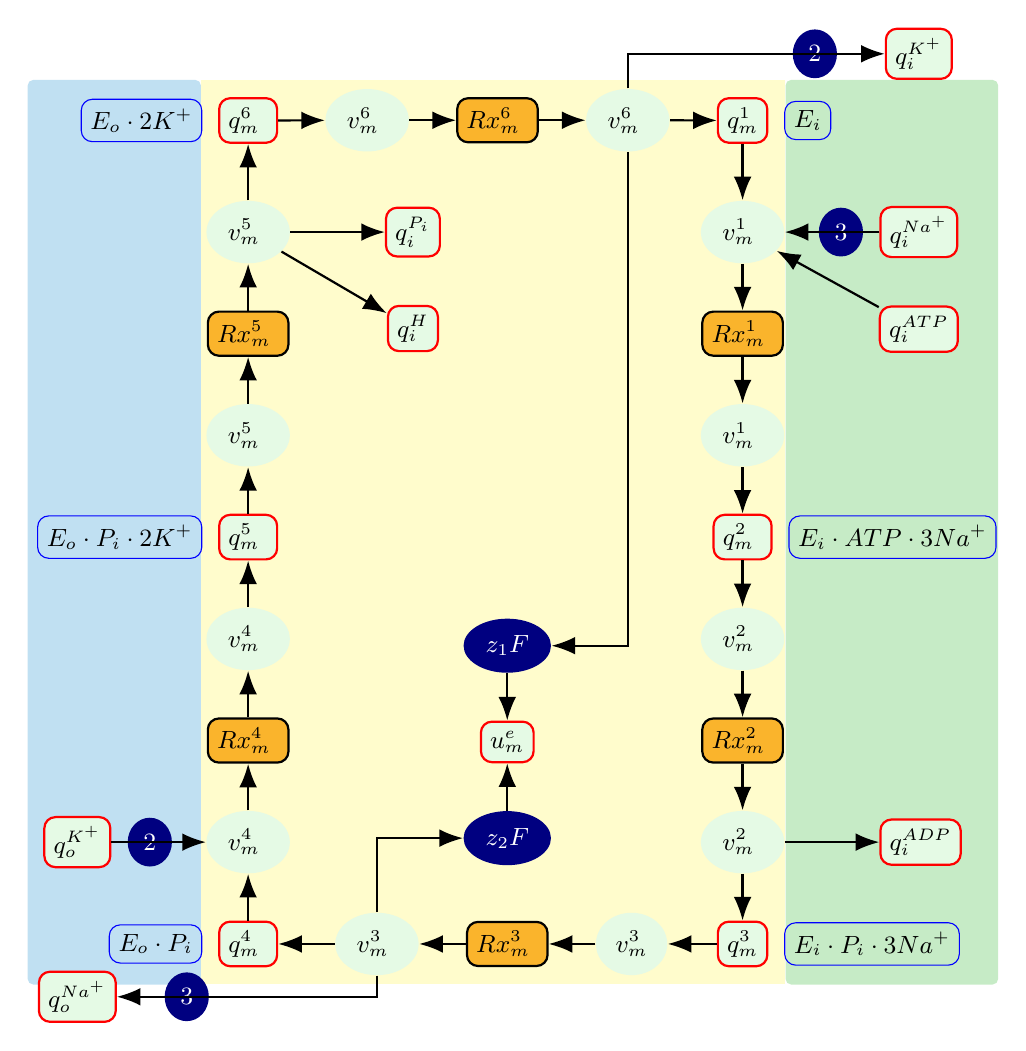
\begin{tikzpicture}[node distance=12mm and 0mm]
% Define the row width (distance between start and end nodes)
\def\rowwidth{60mm}
\def\sep{6mm}
\def\sepp{12mm}
% width of the side bands (change as you like)
\def\bandwidth{22mm}
\matrix (top) [matrix of nodes,column sep=\sep] {
  |[rectred]| $q_m^{6}$ & |[greencycle]| $v_m^{6}$ & |[yellowbox]| $Rx_m^{6}$ & |[greencycle]| $v_m^{6}$ & |[rectred]| $q_m^{1}$\\  
};

\foreach \col/\text in {1/$E_o\cdot 2K^+$}{
  \node[rectblue,left=2mm of top-1-\col] (top2-\col) {\text};
}

\foreach \col/\text in {5/$E_i$}{
  \node[rectblue,right=2mm of top-1-\col] (top2-\col) {\text};
}

\matrix (left) [matrix of nodes,row sep=\sep, matrix anchor=north, below=\sep of top-1-1]  {
|[greencycle]| $v_m^{5}$  \\  |[yellowbox]| $Rx_m^{5}$  \\  |[greencycle]| $v_m^{5}$  \\ |[rectred]| $q_m^{5}$ \\ 
 |[greencycle]| $v_m^{4}$ \\  |[yellowbox]| $Rx_m^{4}$ \\ |[greencycle]| $v_m^{4}$ \\  |[rectred]| $q_m^{4}$  \\ 
};

\foreach \row/\text in {4/$E_o\cdot P_i\cdot 2K^+$, 8/$E_o\cdot P_i$}{
  \node[rectblue,left=2mm of left-\row-1] (left2-\row) {\text};
}

\matrix (right) [matrix of nodes,row sep=\sep, matrix anchor=north, below=\sep of top-1-5]  {
 |[greencycle]| $v_m^{1}$  \\ |[yellowbox]| $Rx_m^{1}$ \\  |[greencycle]| $v_m^{1}$ \\  |[rectred]| $q_m^{2}$ \\ 
 |[greencycle]| $v_m^{2}$ \\  |[yellowbox]| $Rx_m^{2}$ \\ |[greencycle]| $v_m^{2}$ \\  |[rectred]| $q_m^{3}$\\ 
};

\foreach \row/\text in {4/$E_i\cdot ATP\cdot 3Na^+$, 8/$E_i\cdot P_i\cdot 3Na^+$}{
  \node[rectblue,right=2mm of right-\row-1] (right2-\row) {\text};}


\matrix (bottom) [matrix of nodes,column sep=\sep, matrix anchor=west, right=\sep of left-8-1]  {
   |[greencycle]| $v_m^{3}$ & |[yellowbox]| $Rx_m^{3}$ & |[greencycle]| $v_m^{3}$\\
};

\draw[arrow] (left-1-1) -- (top-1-1) ;
\draw[arrow] (top-1-5) -- (right-1-1);
\draw[arrow] (bottom-1-1) -- (left-8-1);
\draw[arrow] (right-8-1) -- (bottom-1-3) ;

\foreach \i in {1,...,4}{
  \pgfmathtruncatemacro{\j}{\i+1} % compute i+1 as integer
  \draw[arrow] (top-1-\i) -- (top-1-\j);
}

\foreach \i in {1,...,2}{
  \pgfmathtruncatemacro{\j}{\i+1} % compute i+1 as integer
  \draw[arrow] (bottom-1-\j) -- (bottom-1-\i);
}
\foreach \i in {1,...,7}{
  \pgfmathtruncatemacro{\j}{\i+1} % compute i+1 as integer
  \draw[arrow] (left-\j-1) -- (left-\i-1);
}
\foreach \i in {1,...,7}{
  \pgfmathtruncatemacro{\j}{\i+1} % compute i+1 as integer
  \draw[arrow] (right-\i-1) -- (right-\j-1);
}

\node[rectred,left=\sepp of left-7-1] (Ko)  {$q_o^{K^+}$} ;
\node[bluecycle,right=2mm of Ko] (zko)   {\textcolor{white}{$2$}} ;
\node[rectred,below=13mm of Ko] (Nao)  {$q_o^{Na^+}$} ;
\node[bluecycle,right=6mm of Nao] (zNao)   {\textcolor{white}{$3$}} ;
\node[rectred,right=\sepp of right-1-1] (Nai)   {$q_i^{Na^+}$} ;
\node[bluecycle,left=2mm of Nai] (z3)   {\textcolor{white}{$3$}} ;
\node[rectred,above=16mm of Nai] (Ki)  {$q_i^{K^+}$} ;
\node[bluecycle,left=6mm of Ki] (zki)   {\textcolor{white}{$2$}} ;
\node[rectred,right=\sepp of left-1-1] (Pi)  {$q_i^{P_i}$} ;
\node[rectred,below=\sep of Pi] (H)  {$q_i^{H}$} ;
\node[rectred,below=\sep of Nai] (ATP)  {$q_i^{ATP}$} ;
\node[rectred,right=\sepp of right-7-1] (ADP)  {$q_i^{ADP}$} ;
\node[rectred,above=20mm of bottom-1-2] (um)  {$u_m^{e}$} ;
\node[bluecycle,above=\sep of um] (z1)  {\textcolor{white}{$z_1F$}} ;
\node[bluecycle,below=\sep of um] (z2)  {\textcolor{white}{$z_2F$}} ;
\draw[arrow] (z1) -- (um);
\draw[arrow] (z2) -- (um);
\draw[arrow] (top-1-4) |- (z1);
\draw[arrow] (bottom-1-1) |- (z2);
\draw[arrow] (Ko) -- (left-7-1);
\draw[arrow] (bottom-1-1) |- (Nao);
\draw[arrow] (top-1-4) |- (Ki);
\draw[arrow] (Nai) -- (right-1-1);
\draw[arrow] (right-7-1) -- (ADP);
\draw[arrow] (left-1-1) -- (Pi);
\draw[arrow] (left-1-1) -- (H);
\draw[arrow] (ATP) -- (right-1-1);

%=========================
% Background shading
%=========================
\begin{scope}[on background layer]
  \node[fit=(top-1-1)(right-8-1), fill=yellow!20, inner sep=6pt] (fitnode) {};
% Right band: from fitnode.south east to fitnode.north east shifted right by \bandwidth
    \fill[LimeGreen!80!gray!30, rounded corners=2pt]
      (fitnode.south east) rectangle ($ (fitnode.north east) + (27mm,0) $);
    % Left band: from fitnode.south west shifted left by \bandwidth to fitnode.north west
    \fill[Cerulean!80!gray!30, rounded corners=2pt]
      ($ (fitnode.south west) + (-\bandwidth,0) $) rectangle (fitnode.north west);
\end{scope}


\end{tikzpicture}
\end{document}
